\newpage
\section{Implementierung}

TODO:

Umsetzung der Anforderung X.X "Erkennen des Ziels mit einer Abweichung von einem Meter".
Dieser Abschnitt erläutert die Umsetzung der Anforderung X.X. Wie bereits beschrieben wird GPS zur Abstandsermittlung verwendet. Das bedeutet, während der Nutzer sich auf das Ziel zubewegt wird der Standort über GPS bestimmt. Bereits in Kapitel X ist die Genauigkeit von GPS Positionen angegeben.  Sie liegt bei x Metern. Um mit dieser Genauigkeit erkennen zu können, ob sich ein Spieler am Ziel befindet wurde ein Radius von 10 Metern um den Zielpunkt gewählt. Nach einigen Praxistests wurde deutlich, dass dieser Radius nicht ausreicht. Die Testkandidaten konnten den Zielpunkt trotz des Radiuses nicht erreichen. Aus diesem Grund entschied man sich dazu die Genauigkeit am Zielpunkt deutlich zu erhöhen. Zum Einsatz kommen iBeacons. In Kapitel X ist bereits auf RadioButtons eingegangen worden. Eine Unterkategorie bilden die iBeacons.

iBeacons

Bei iBeacons handelt es sich um eine neue Technologie zur Abstands bzw. Standortbestimmung von Smartphones welche vom Hersteller Apple stammt. Auf Materieller Ebene betrachtet ist ein iBeacon ein kleines Gerät welches ständig Bluetooth Signale sendet. Die verwendete Technik ist Bluetooth Low Energy (BLE). Das Gerät besteht aus

einer kleinen Platine mit Bluetooth-Sender und einer Knopfzelle. Beides steckt in einem Kunststoffgehäuse, das in der Größe zwischen einem dicken 2-Euro-Stück und einer PC-Maus rangiert.

http://www.golem.de/news/bluetooth-low-energy-ibeacon-ist-mehr-als-ein-leuchtfeuer-1403-105331-2.html

Übertragen werden mit dem Signal nur eine ID sowie drei Zahlen. Vorteil der BLE Technologie ist der geringe Stromverbrauch. Laut Hersteller soll ein iBeacon zwischen sechs und vierundzwanzig Monaten ein Signal senden können. Abhängig ist dies von der Signalstärke und dem Sendeintervall. Mit dem 2,4 GHz Signal werden Reichweiten von bis zu 50 Metern erreicht. Ein Smartphones welches das Signal empfängt kann einen ungefähren Abstand zum iBeacon ermitteln. Verwendet man mehrere iBeacons, kann über Triangulation ein genauer Standort bestimmt werden. Besonders an dieser Standortbestimmung ist, dass sie auch in Gebäuden funktioniert. Hier ist GPS teilweise gar nicht oder nur schlecht empfangbar. Daraus resultieren diverse Anwendungsbereich im folgenden sind ein paar aufgelistet:

\begin{description}
\item[$\bullet$]die Navigation und Präsentation von Informationen im Museum

\item[$\bullet$]das Dirigieren von Bahnfahrern zum richtigen Bahnsteig und Wagen

\item[$\bullet$]Rabattprogramme und Kundenkarten

\item[$\bullet$]Abholbenachrichtigungen für vorbestellte Waren beim Betreten des Ladens

\item[$\bullet$]die Automatisierung von Gebäudefunktionen wie Heizung, Licht und Jalousiestellung

\item[$\bullet$]Hinweise auf die Stadion-Einlasskontrolle mit den kürzesten Wartezeiten

\item[$\bullet$]Live-Umfragen unter Teilnehmern einer Vortragsveranstaltung

\item[$\bullet$]kostenlose Lektüre einer Zeitschrift beim Aufenthalt in einem Café

\item[$\bullet$]Bereitstellung der Tageskarte eines Restaurants auf dem Smartphone

\end{description}

http://www.golem.de/news/bluetooth-low-energy-ibeacon-ist-mehr-als-ein-leuchtfeuer-1403-105331.html

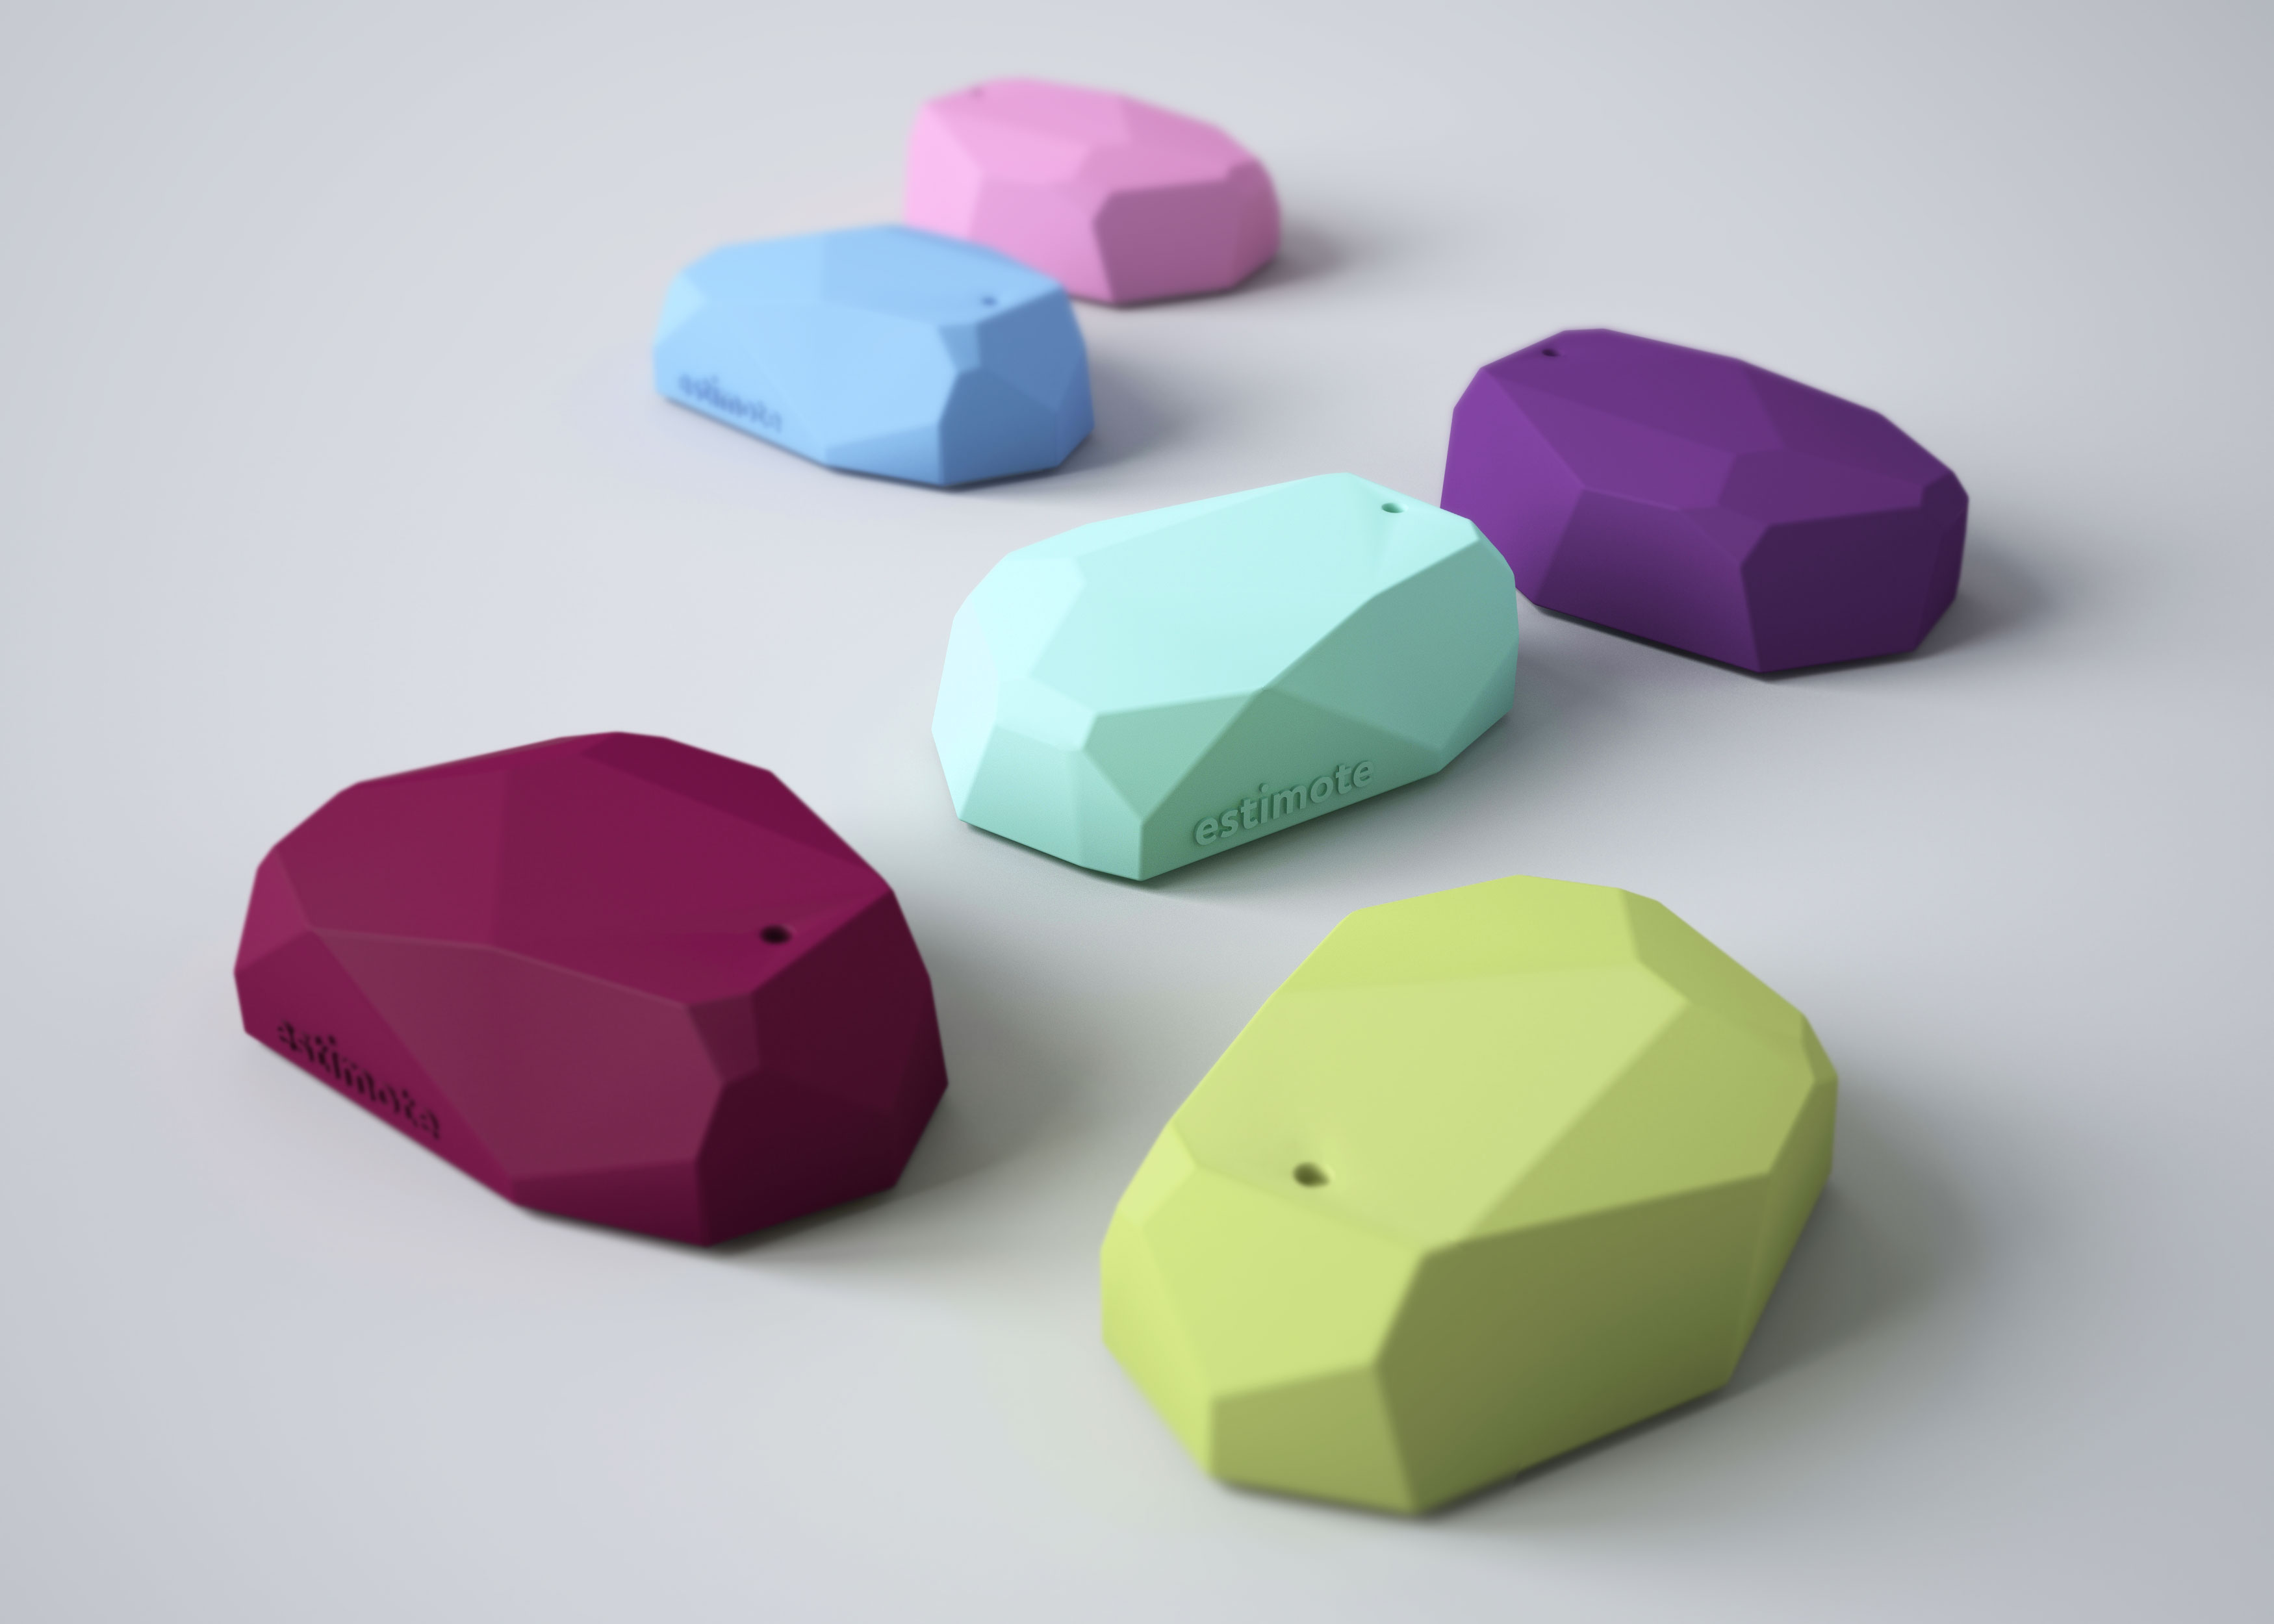
\includegraphics[width=0.5\textwidth]{ref/images/ibeacon.jpg}
iBeacons der Firma Estimote

Empfangen werden können die Signale der iBeacons mit Bluetooth 4.0 Empfangsmodulen. Hierzu zählen die aktuelle Smartphones. Dies funktioniert sowohl mit Apple sowie Android Geräten, was für diese Arbeit von großer Bedeutung ist.



 